\documentclass{article}
%%%%%%%%%%%%%%%%%%%%%%%%%%%%%%%%%%%%%%%%%%%%%%%%%%%%%%%%%%%%%%%%%%%%%%%%%%%%%%%
% PREAMBLE
%%%%%%%%%%%%%%%%%%%%%%%%%%%%%%%%%%%%%%%%%%%%%%%%%%%%%%%%%%%%%%%%%%%%%%%%%%%%%%%
\usepackage{mathtools}
\usepackage{algorithm}
\usepackage{algorithmic}
\usepackage{fancyvrb}
\usepackage{booktabs}
\usepackage{rotating}
\usepackage{tikz}
\usepackage{float}
\usepackage{hyperref}
\usepackage{subcaption}
\usetikzlibrary{arrows,decorations.pathmorphing,backgrounds,positioning,fit,matrix}
\newcommand{\DepProps}{\textsc{DepProps}}
\usepackage{titling}
\newcommand{\subtitle}[1]{%
  \posttitle{%
    \par\end{center}
    \begin{center}\large#1\end{center}
    \vskip0.5em}%
}
\begin{document}
% TITLE
\title{DM819 - Computational Geometry}
\subtitle{Fall 2015\\Project 2}
% AUTHER
\author{Mikkel Levisen and Jesper Lund}
%DATE
\maketitle
% no page number on first page
\thispagestyle{empty}
\newpage
% TABLE OF CONTENTS
\tableofcontents
% no page number on table of contents page
\thispagestyle{empty}
\newpage
% restart page number counter
\pagenumbering{arabic} 
%%%%%%%%%%%%%%%%%%%%%%%%%%%%%%%%%%%%%%%%%%%%%%%%%%%%%%%%%%%%%%%%%%%%%%%%%%%%%%%
% DOCUMENT START
%%%%%%%%%%%%%%%%%%%%%%%%%%%%%%%%%%%%%%%%%%%%%%%%%%%%%%%%%%%%%%%%%%%%%%%%%%%%%%%
\section{Introduction}
  This report details the implementation of KD-Tree and Range-Tree for 
  $n$-dimensional input. Each tree is constructed from a list of unsorted points
  and is capable of performing orthogonal range queries.
\section{Range Queries}

  A point $p \in P$ exists in the range $R$ iff.
  \[
    \forall p_i \in p: \{ R_{i,1}\leq   p_i \leq R_{i,2}\}|\forall i \in \{1,...,n\}, n = dimensions 
  \]

  A range query consists of reporting all points, $p$, which lie within a given 
  range, $R$.
  An $n$-dimensional point, $P_n$, consist of real numbers 
  $\{p_1,p_2,\dots,p_n\}$, and an $n$-dimensional range $R_n$ consist of 
  $[x:x']\times[y:y'] \times \dots \times[z:z']$. A range query consist of 
  reporting all points $P_n$ in a range $R_n$.
\section{KD-Tree}
\subsection{Complexity}
\section{Range-Tree}
  A Range-tree is a multi-level data structure for time efficient range queries.
  An $n$-dimensional Range-tree consist of $n$ levels where each level, $l$, is 
  a 1-dimensional range query on the $l$'th  
  determining 
  canonical subset $P(v)$
  associated structure
  n-level tree
\subsection{Complexity}
\section{Test}
  \subsection{Test Generation}
    Supplied with the code is a test generating script which can create tests of
    arbitrary dimension and size. The tests are sorted in directories by 
    dimension.
    
    In a tests consisting of $n$ points in $d$ dimensions an $d$-dimensional 
    volume is constructed with a side length $s = \sqrt[d]{n}$. For each such 
    volume is $1000$ ranges generated with a side length of 
    $rs = \sqrt[d]{0.1 \cdot s^d}$ i.e. each range will contain approximately 
    10\% of the $n$ points. 
    
    The generated tests also contains the correct output of each range query.
    
  %  $ $1/10$ the size of the    
    
%   In each test are points randomly uniformly distributed in $n$ dimensions by 
%   constructing an $n$-dimensional volume with a 
% D = {1,2,3,4,5,6}
%-- number of ranges
%R = {1000}
%-- size of dimensions
%S = function(n,d) return n^(1/d) end
%-- range sizes
%range volume
%$$
%  \sqrt[d]{n}
%$$
%
%
%$$
%  
%$$
%$s=$range side  
\begin{figure}[H]
    \centering
    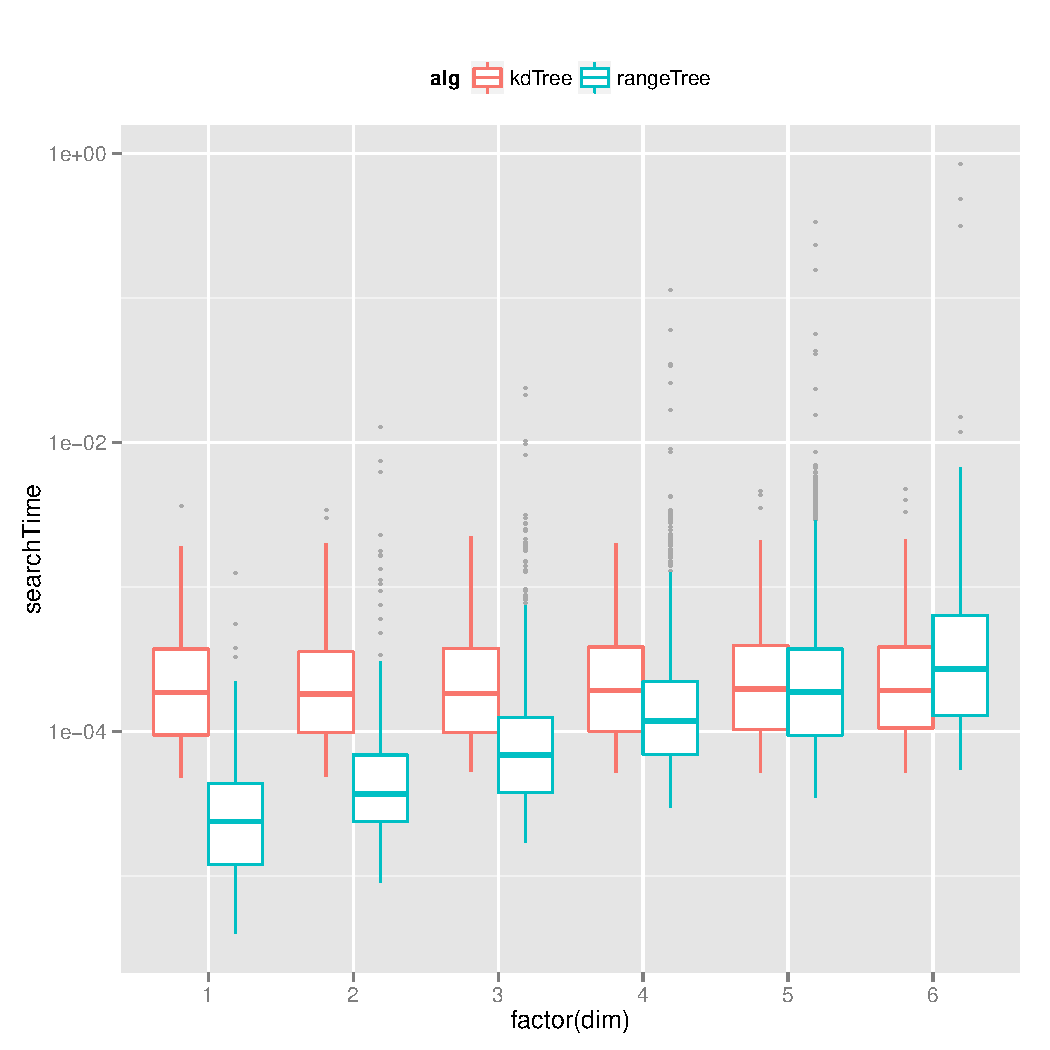
\includegraphics[width=\textwidth]{../src/R/plots/boxplot.pdf}
\end{figure}
\begin{figure}[H]
    \centering
    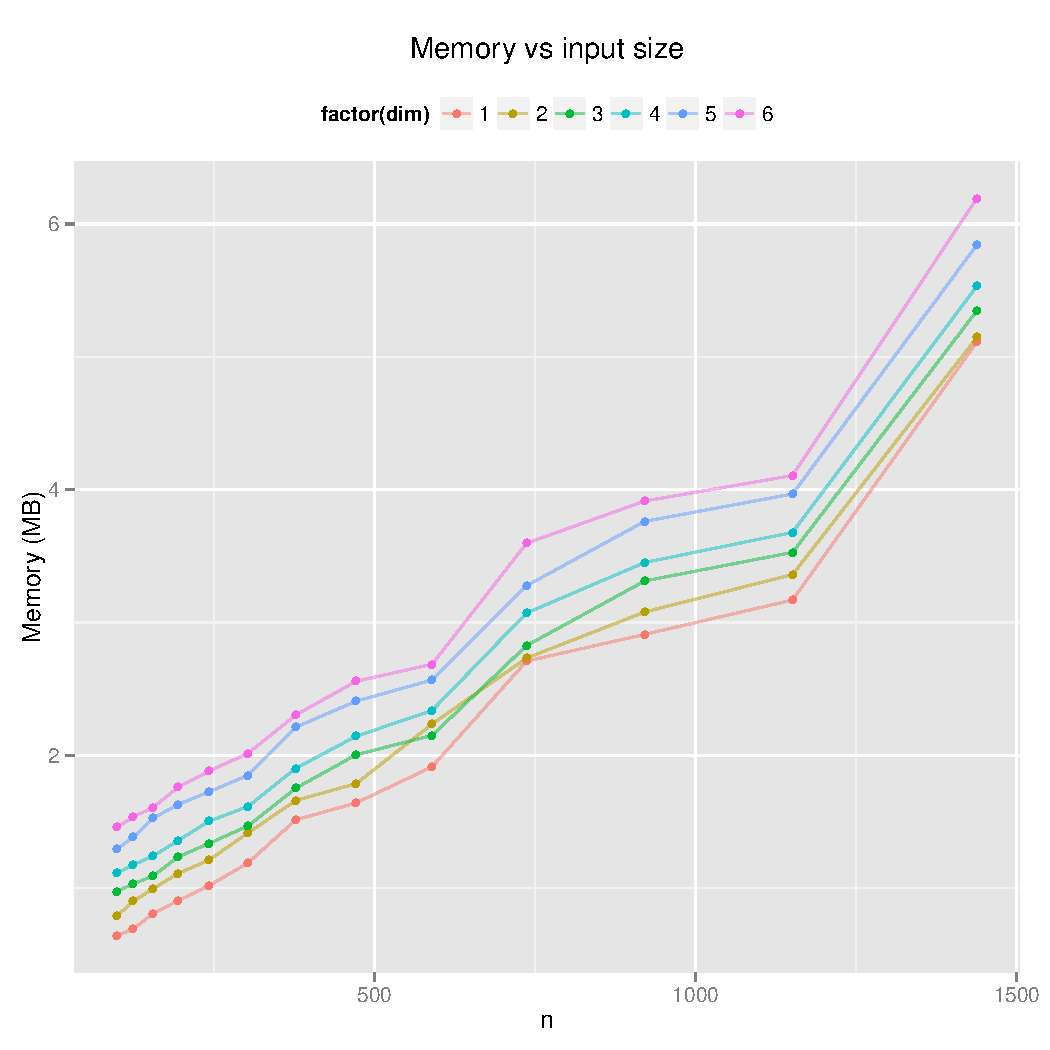
\includegraphics[width=\textwidth]{../src/R/plots/kdmem.pdf}
\end{figure}
\begin{figure}[H]
    \centering
    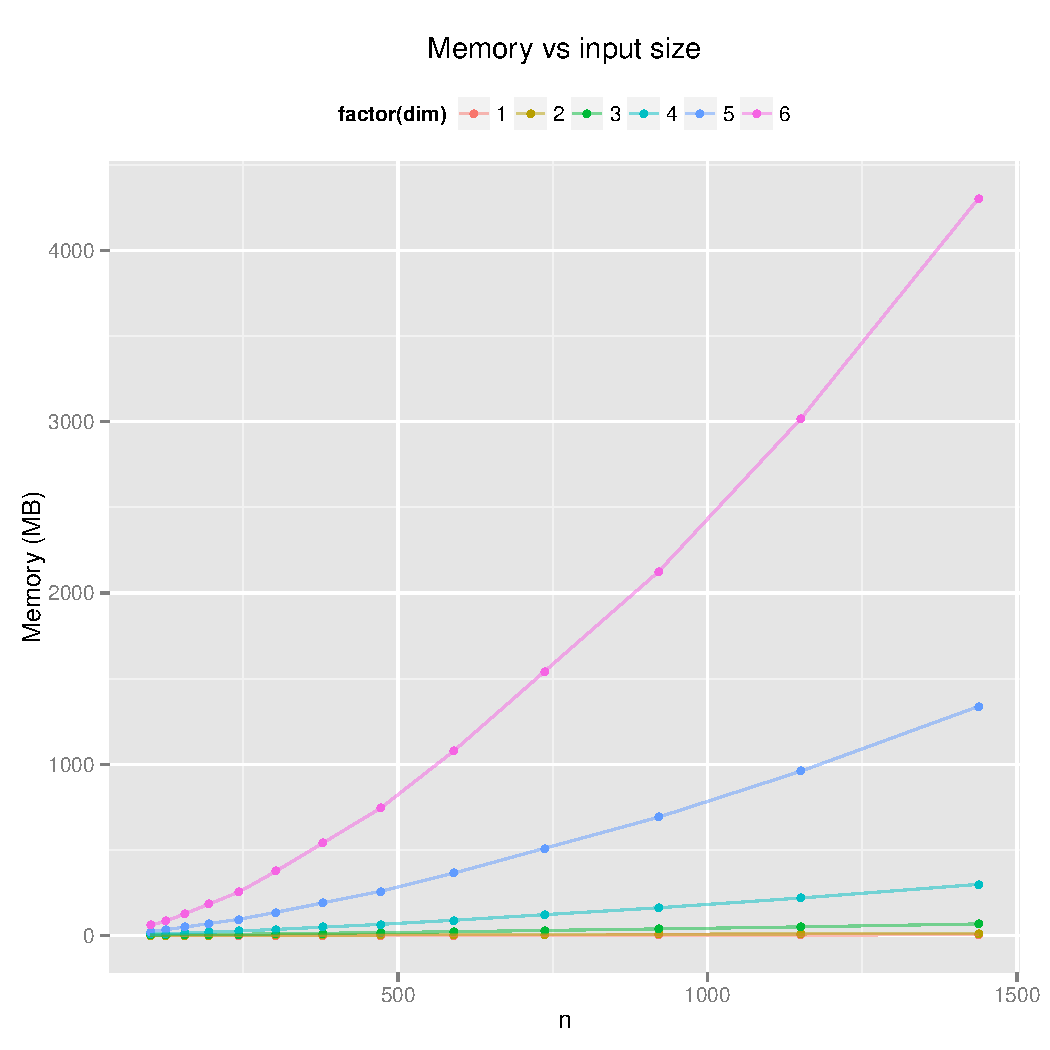
\includegraphics[width=\textwidth]{../src/R/plots/rtmem.pdf}
\end{figure}
\section{Manual}
  \subsection{File Formats}
  \begin{verbatim}
  	<real> \t <real>
  	<real> \t <real>
  	<real> \t <real>
  	<real>:<real> \t <real>:<real> , <integer> \t <integer>
  	<real>:<real> \t <real>:<real> , <integer> \t <integer>
  	<real>:<real> \t <real>:<real>
  \end{verbatim}

  \subsection{Inscrutions}
\subsection{File Structure}
\begin{verbatim}
ROOT
|-- report/
`-- src
    |-- kdtree
    |   |-- inspect.lua
    |   |-- kdtree.lua
    |   `-- test.lua
    |-- R
    |   `-- makePlots.R
    |-- rangeTree
    |   |-- inspect.lua
    |   |-- middleclass
    |   |   `-- middleclass.lua
    |   |-- RangeTree.lua
    |   `-- test.lua
    |-- results/
    |-- runTests.py
    `-- tests
        |-- createCustomTest.lua
        |-- dimension_1/
        |-- dimension_2/
        |-- dimension_3/
        |-- dimension_4/
        |-- dimension_5/
        |-- dimension_6/
        |-- genTestSuite.lua
        `-- inspect.lua
\end{verbatim}

\section{Conclusion}
\end{document}